\documentclass[reqno]{amsart}
\usepackage{amscd, amssymb, amsmath, amsthm}
\usepackage{graphicx}
\usepackage[colorlinks=true,linkcolor=blue]{hyperref}
\usepackage[utf8]{inputenc}
\usepackage[T1]{fontenc}
\usepackage{textcomp}
\usepackage{babel}
%% for identity function 1:
\usepackage{bbm}
%%For category theory diagrams:
\usepackage{tikz-cd}

%\usepackage[backend=biber]{biblatex}
%\addbibresource{.bib}


\setlength\parindent{0pt}

\pdfsuppresswarningpagegroup=1

\newtheorem{theorem}{Theorem}[section]
\newtheorem{lemma}[theorem]{Lemma}
\newtheorem{proposition}[theorem]{Proposition}
\newtheorem{corollary}[theorem]{Corollary}
\newtheorem{conjecture}[theorem]{Conjecture}

\theoremstyle{definition}
\newtheorem{definition}[theorem]{Definition}
\newtheorem{example}[theorem]{Example}
\newtheorem{exercise}[theorem]{Exercise}
\newtheorem{problem}[theorem]{Problem}
\newtheorem{question}[theorem]{Question}

\theoremstyle{remark}
\newtheorem*{remark}{Remark}
\newtheorem*{note}{Note}
\newtheorem*{solution}{Solution}
\newtheorem*{construction}{Construction}



%Inequalities
\newcommand{\cycsum}{\sum_{\mathrm{cyc}}}
\newcommand{\symsum}{\sum_{\mathrm{sym}}}
\newcommand{\cycprod}{\prod_{\mathrm{cyc}}}
\newcommand{\symprod}{\prod_{\mathrm{sym}}}

%Linear Algebra

\DeclareMathOperator{\Span}{span}
\DeclareMathOperator{\im}{im}
\DeclareMathOperator{\diag}{diag}
\DeclareMathOperator{\Ker}{Ker}
\DeclareMathOperator{\ob}{ob}
\DeclareMathOperator{\Hom}{Hom}
\DeclareMathOperator{\Mor}{Mor}
\DeclareMathOperator{\sk}{sk}
\DeclareMathOperator{\Vect}{Vect}
\DeclareMathOperator{\Set}{Set}
\DeclareMathOperator{\Group}{Group}
\DeclareMathOperator{\Ring}{Ring}
\DeclareMathOperator{\Ab}{Ab}
\DeclareMathOperator{\Top}{Top}
\DeclareMathOperator{\hTop}{hTop}
\DeclareMathOperator{\Htpy}{Htpy}
\DeclareMathOperator{\Cat}{Cat}
\DeclareMathOperator{\CAT}{CAT}
\DeclareMathOperator{\Cone}{Cone}
\DeclareMathOperator{\dom}{dom}
\DeclareMathOperator{\cod}{cod}
\DeclareMathOperator{\Aut}{Aut}
\DeclareMathOperator{\Mat}{Mat}
\DeclareMathOperator{\Fin}{Fin}
\DeclareMathOperator{\rel}{rel}
\DeclareMathOperator{\Int}{Int}
\DeclareMathOperator{\sgn}{sgn}
\DeclareMathOperator{\Homeo}{Homeo}
\DeclareMathOperator{\SHomeo}{SHomeo}
\DeclareMathOperator{\PSL}{PSL}
\DeclareMathOperator{\Bil}{Bil}
\DeclareMathOperator{\Sym}{Sym}
\DeclareMathOperator{\Skew}{Skew}
\DeclareMathOperator{\Alt}{Alt}
\DeclareMathOperator{\Quad}{Quad}
\DeclareMathOperator{\Sin}{Sin}
\DeclareMathOperator{\Supp}{Supp}
\DeclareMathOperator{\Char}{char}
\DeclareMathOperator{\Teich}{Teich}
\DeclareMathOperator{\GL}{GL}
\DeclareMathOperator{\tr}{tr}
\DeclareMathOperator{\codim}{codim}
\DeclareMathOperator{\coker}{coker}
\DeclareMathOperator{\corank}{corank}
\DeclareMathOperator{\rank}{rank}
\DeclareMathOperator{\Diff}{Diff}
\DeclareMathOperator{\Bun}{Bun}
\DeclareMathOperator{\Sm}{Sm}
\DeclareMathOperator{\Fr}{Fr}
\DeclareMathOperator{\Cob}{Cob}
\DeclareMathOperator{\Ext}{Ext}
\DeclareMathOperator{\Tor}{Tor}
\DeclareMathOperator{\Conf}{Conf}
\DeclareMathOperator{\UConf}{UConf}
\DeclareMathOperator{\Map}{Map}



%Row operations
\newcommand{\elem}[1]{% elementary operations
\xrightarrow{\substack{#1}}%
}

\newcommand{\lelem}[1]{% elementary operations (left alignment)
\xrightarrow{\begin{subarray}{l}#1\end{subarray}}%
}

%SS
\DeclareMathOperator{\supp}{supp}
\DeclareMathOperator{\Var}{Var}

%NT
\DeclareMathOperator{\ord}{ord}

%Alg
\DeclareMathOperator{\Rad}{Rad}
\DeclareMathOperator{\Jac}{Jac}

%Misc
\newcommand{\SL}{{\mathrm{SL}}}
\newcommand{\mobgp}{{\mathrm{PSL}_2(\mathbb{C})}}
\newcommand{\id}{{\mathrm{id}}}
\newcommand{\MCG}{{\mathrm{MCG}}}
\newcommand{\PMCG}{{\mathrm{PMCG}}}
\newcommand{\SMCG}{{\mathrm{SMCG}}}
\newcommand{\ud}{{\mathrm{d}}}
\newcommand{\Vol}{{\mathrm{Vol}}}
\newcommand{\Area}{{\mathrm{Area}}}
\newcommand{\diam}{{\mathrm{diam}}}
\newcommand{\End}{{\mathrm{End}}}


\newcommand{\reg}{{\mathtt{reg}}}
\newcommand{\geo}{{\mathtt{geo}}}

\newcommand{\tori}{{\mathcal{T}}}
\newcommand{\cpn}{{\mathtt{c}}}
\newcommand{\pat}{{\mathtt{p}}}

\let\Cap\undefined
\newcommand{\Cap}{{\mathcal{C}}ap}
\newcommand{\Push}{{\mathcal{P}}ush}
\newcommand{\Forget}{{\mathcal{F}}orget}




\begin{document}

\section{Hatcher}
    In this section, we will cover the cup product following Hatcher.\\

    \begin{definition}[Cup Product]
        For a ring $R$, let
        $\varphi \in C^{k}(X;R)$ and
        $\psi \in C^{l}(X;R)$. Then
        the \textit{cup product}
        $\varphi \smile \psi \in C^{k+l}(X;R)$ is the cochain
        whose value
        on $\sigma \colon \Delta^{k+l} \to X$ is given
        by
        \[
            \left( \varphi \smile \psi  \right) (\sigma)
            = \varphi \left( \sigma |_{\left[ v_0,\ldots,
            v_k \right] } \right) 
            \psi \left( \sigma|_{\left[ v_k,\ldots,
            v_{k+l} \right] } \right) 
        \] 
        where the right-hand side is the product
        in $R$.
    \end{definition}

    To see that this induces a
    cup product on cohomology, we
    need the following lemma:

    \begin{lemma}[]
        $\delta \left( \varphi \smile
        \psi \right) = 
        \delta \varphi \smile \psi +
        (-1)^{k} \varphi \smile \delta \psi $ 
        for $\varphi \in C^{k}(X;R)$ and
        $\psi \in C^{l}(X;R)$.
    \end{lemma}

    Using the lemma, it is clear
    that the cup product
    of two cocycles is again a cocycles, and
    that the cup product of a
    cocycle and a coboundary, in either order,
    is a coboundary.
    It follows that there is an induced cup product
    \[
    H^{k}(X;R) \times H^{l}(X;R)
    \stackrel{\smile}{\to} H^{k+l}(X;R).
    \] 
    This is associative and distributive since at the level
    of cochains the cup product has these properties.\\
    If $R$ has an identity, then there is an identity
    elements for the cup product, the class
    $1 \in H^{0}(X;R)$ defined by the
    $0$-cocycle taking the value $1$ on each singular
    $0$-simplex.

    \subsubsection{Relative cup product}
    The cup product formula $\left( \varphi \smile
    \psi \right) (\sigma) = 
    \varphi \left( \sigma |_{\left[ v_0, \ldots, v_k \right] 
    }\right) \psi \left( 
    \sigma |_{\left[ v_k, \ldots, v_{k+l} \right] }\right) $ also
    gives relative cup products
    \begin{align*}
        H^{k}(X;R) \times H^{l}(X,A;R)
        &\stackrel{\smile}{\to} H^{k+l}(X,A;R)\\
        H^{k}(X,A;R) \times H^{l}(X;R)
        &\stackrel{\smile}{\to} H^{k+l}(X,A;R)\\
        H^{k}(X,A;R) \times H^{l}(X,A;R)
        &\stackrel{\smile}{\to} H^{k+l}(X,A;R)
    \end{align*}
    since if $\varphi $ or $\psi $ vanishes
    on chains in $A$, then so does
    $\varphi \smile \psi $.\\
    \linebreak
    We can also define an even more general relative cup product
    \[
    H^{k}(X,A;R) \times H^{l}(X,B;R)
    \stackrel{\smile}{\to} H^{k+l}(X, A \cup B;R)
    \] 
    when $A$ and $B$ are open subsets of $X$ or subcomplexes
    of the CW complex $X$.

    \begin{construction}
        The absolute cup product restricts to a cup product
        $C^{k}(X,A;R) \times C^{l}(X,B;R)
        \to C^{k+l}(X,A \sqcup  B; R)$ where
        $C^{n}\left( X,A \sqcup  B;R \right) $ is the subgroup
        of $C^{n}(X;R)$ consisting of cochains vanishing
        on sums of chains in $A$ and chains in $B$.
        If $A$ and $B$ are open in $X$, then
        the inclusions
        $C^{n} (X,A \cup B;R) \hookrightarrow 
        C^{n}(X, A\sqcup B;R)$ induces
        isomorphisms on cohomology:
        
    \end{construction}











    \begin{proposition}[]
        For a map $f \colon X \to Y$, the induced
        map $f^{*} \colon
        H^{n} (Y;R) \to H^{n}(X;R)$ satisfies
        $f^{*}\left( \alpha \smile \beta \right) 
        = f^{*}(\alpha) \smile
        f^{*}(\beta)$, and similarly in the relative
        case.
    \end{proposition}

    \begin{theorem}[]
        The identity $\alpha \smile \beta =
        (-1)^{kl} \beta \smile \alpha$ holds
        for all $\alpha \in H^{k}\left( X,A;R \right) $ and
        $\beta \in H^{l}(X,A;R)$, when $R$ is commutative.
    \end{theorem}

    \section{The Cohomology Ring}

    Since the cup product is associative and distributive,
    it is natural to try to make it the
    multiplication in a ring structure on
    the cohomology groups of a space $X$.
    This is easy to do if we define
    $H^{*}(X;R) = \bigoplus_{k \in \mathbb{Z}} H^{k}(X;R)$.
    That is, if we define $H^{*}(X;R)$ as the
    direct sum of the cohomology
    groups of the space. Then
    elements of $H^{*}(X;R)$ are
    finite sums
    $\Sigma_i \alpha_i$ with
    $\alpha_i \in H^{i}(X;R)$ and the
    product of two such sums
    is defined to be
    $\left( \Sigma_i \alpha_i \right) 
    \left( \Sigma_j \beta_j \right) =
    \Sigma_{i,j} \alpha_i \beta_j$.
    
    \begin{exercise}[]
        Show that this makes $H^{*}(X;R)$ into a ring,w
        with identity if $R$ has an identity.
        Similarly for $H^{*}(X,A;R)$ with the relative
        cup product.

        Taking scalar multiplication by elements
        of $R$ into account, these rings
        can also be regarded as $R$-algebras.
    \end{exercise}

    \begin{example}[]
        Recall that
        $H^{k}(\mathbb{R}\mathbb{P}^{2};\mathbb{Z}_2)
        \cong \mathbb{Z}_2$ for
        $k = 0, 1,2$ and is $0$ otherwise.
        Also by example 3.8 in Hatcher on Cohomology,
        for a generator
        $\alpha \in H^{1}(\mathbb{R}\mathbb{P}^2;\mathbb{Z}_2)$,
        $\alpha^2 
        =\alpha \smile \alpha$ is a generator
        of $H^{2}(\mathbb{R}\mathbb{P}^2; \mathbb{Z}_2)$,
        hence
        $H^{*}(\mathbb{R}\mathbb{P}^2;\mathbb{Z}_2) \cong
        \mathbb{Z}_2 \left[ \alpha \right] /
        \left( \alpha^3 \right) $.
    \end{example}

    Adding cohomology classes of different dimensions
    to form $H^{*}(X;R)$ is convenient, but it has
    little topological significance. One
    can always regard the
    cohomology ring as a \textit{graded ring}:

    \begin{definition}[Graded Ring]
        A ring $A$ with a decomposition
        $\bigoplus_{k\ge 0}A_k$  into additive
        subgroups $A_k \le A$ such that the
        multiplication takes
        $A_k \times A_l$ to $A_{k+l}$ is called
        a \textit{graded ring}.
    \end{definition}

    To indicate that $\alpha \in A$ lies
    in $A_k$, we write
    $\left| a \right| = k$.

    \begin{definition}[Degree/dimension]
        The number $\left| a \right| $ 
        is called the \textit{degree} or 
        \textit{dimension} of $a$.
    \end{definition}

    \begin{definition}[Commutative/anticommutative/graded commutative]
        A graded ring satisfying the commutativity
        property that
        $ab = (-1)^{\left| a \right| \left| b \right| } ba$ 
        is usually called \textit{commutative} or any of
        the following less ambiguous terms:
        \textit{graded commutative},
        \textit{anticommutative}, or 
        \textit{skew commutative}.
    \end{definition}

    \begin{example}[Polynomial Rings]
        An example of a graded ring is
        $R \left[ \alpha \right] $ or
        the truncated version: $R \left[ \alpha \right] /
        \left( \alpha^n \right) $.

        We have seen that
        $H^{*}\left( \mathbb{R}\mathbb{P}^{2}; \mathbb{Z}/2 \right) 
        \cong \mathbb{Z}/2 \left[ \alpha \right] /
        \left( \alpha^{3} \right) $.
        More generally, we can show that
        $H^{*}\left( \mathbb{R}\mathbb{P}^{n};
        \mathbb{Z}/2\right) \cong
        \mathbb{Z}/2 \left[ \alpha \right] /
        \left( \alpha^{n+1} \right) $ and
        $H^{*}\left( \mathbb{R}\mathbb{P}^{\infty};
        \mathbb{Z}/2\right) \cong
        \mathbb{Z}/2 \left[ \alpha \right] $, where,
        in these cases, $\left| \alpha \right| = 1$.
    \end{example}

    \begin{example}[Exterior Algebras]
        The \textit{exterior algebra}
        $\Lambda_R \left[ \alpha_1, \ldots, \alpha_n \right] $ 
        over a commutative ring $R$ with identity
        is the free $R$-module with basis
        the finite products
        $\alpha_{i_1} \cdots \alpha_{i_k},
        i_1 < \ldots < i_k$, with associative,
        distributive multiplication defined by
        the rules
        $\alpha_i \alpha_j = - \alpha_j \alpha_i$ for
        $i\neq j$ and
        $\alpha_i^2 = 0$ for all $i$.
        The empty producto f $\alpha_i$ 's is the identity
        element $1$ in
        $\Lambda_R \left[ \alpha_1, \ldots, \alpha_n \right] $.

        In view of
        $\alpha_i \alpha_j = - \alpha_j \alpha_i$,
        the exterior algebra becomes an
        anticommutative graded ring by specifying
        odd dimensions for the generators
        $\alpha$.

        By the Künneth formula, we have
        \[
        H^{*}\left( S^{k_1} \times 
        \ldots \times S^{k_n} ; \mathbb{Z}\right) 
        \cong
        H^{*}(S^{k_1} ; \mathbb{Z}) \otimes_{\mathbb{Z}} \ldots
        \otimes_{\mathbb{Z}} H^{*}(S^{k_n};\mathbb{Z})
        \cong \Lambda_{\mathbb{Z}}
        \left[ \alpha_1, \ldots, \alpha_n \right] 
        \] 
        when all the $k_i$ are odd,
        since the first isomorphism
        is given by the cross product.

        When some $k_i$ 's are even, one obtains
        the tensor product of an exterior algebra
        for the odd-dimensional speheres and truncated
        polynomial rings
        $\mathbb{Z} \left[ \alpha \right] /
        \left( \alpha^2 \right) $ for the even
        dimensional spheres.
    \end{example}

    \subsection{The Cross Product}
    
    \begin{definition}[First definition of cross product,
        external cup product]
        We define the \textit{cross product}, or
        \textit{external cup product} as it is
        sometimes called, by
        the map
        \[
        H^{*}(X;R) \times H^{*}(Y;R) \stackrel{\times }{\to} 
        H^{*}\left( X \times Y; R \right) 
        \] 
        given by
        $a \times b = p_1^{*}(a) \smile p_2^{*}(b)$ where
        $p_1, p_2$ are the projections of
        $X \times Y$ onto $X$ and $Y$, respectively.
    \end{definition}

    \begin{definition}[Cross Product, second definition]
    Since the cup product is distributive, the cross
    product is bilinear, hence it induces an
    $R$-module homomorphism

    \begin{equation*}
    \begin{tikzcd}
        H^{*}(X;R) \times H^{*}(Y;R) \ar[dr, "\times "]
        \ar[d] &\\
        H^{*}(X;R) \otimes_R H^{*}(Y;R) 
        \ar[r, "\times "] & H^{*}(X \times Y;R)
    \end{tikzcd}
    \end{equation*}
    which we also call the cross product, given
    by $a \otimes b \mapsto a \times b$.
    \end{definition}

    This module homomorphism becomes
    a ring homomorphism if we define
    the multiplication in a tensor product
    of graded rings by
    $\left( a \otimes b \right) \left( c \otimes d \right) 
    = (-1)^{\left| b \right| \left| c \right| }
    ac \otimes bd$ where
    $\left| x \right| $ denotes the dimension of $x$.
    
    This can be seen as follows (note that
    $ac = a \smile c$ and $bd = b \smile d$ ):
    \begin{align*}
        \mu \left( \left( a \otimes b \right) 
        \left( c \otimes d \right) \right) 
        &= (-1)^{\left| b \right| \left| c \right| }
        \mu \left( ac \otimes bd \right) \\
        &= (-1)^{\left| b \right| \left| c \right| }
        (a \smile c) \times (b \smile d)\\
        &= (-1)^{\left| b \right| \left| c \right| }
        p_1^{*} (a \smile c) \smile
        p_2^{*}\left( b \smile d \right) \\
        &= (-1)^{\left| b \right| \left| c \right| }
        p_1^{*}(a) \smile p_1^{*}(c) \smile
        p_2^{*}(b) \smile p_2^{*}(d)\\
        &= p_1^{*}(a) \smile p_2^{*}(b) \smile
        p_1^{*}(c) \smile p_2^{*}(d)\\
        &= \left( a \times b \right) \left( c
        \times d\right) = \mu (a \otimes b) 
        \mu (c \otimes d)
    \end{align*}



    \begin{theorem}[]
        The cross product $H^{*}(X;R) \otimes_R
        H^{*}(Y;R) \to H^{*}(X \times Y; R)$ is an
        isomorphism of rings
        if $X$ and $Y$ are CW complexes and
        $H^{k}(Y;R)$ is a finitely generated
        free $R$-module for all $k$.
    \end{theorem}
    
\section{Bredon}


We will need to define a homomorphism
$D \colon \Delta_{n-1}(X) \to \Delta_n(X)$ with some desirable
properties, so let us start with that.
To this end, we construct it in the proof of the following theorem:

\begin{theorem}[]\label{Thm:OOCPPX}
    If $X$ is contractible, then $H_i(X) = 0$ for all
    $i \neq 0$.
\end{theorem}

\begin{proof}
    Let $F \colon X \times I \to X$ be the homotopy with
    $F(x,0) = x$ and $F(x,1) = x_0$ for all $x \in X$, and
    some $x_0 \in X$.
    Define $D \sigma \colon \Delta_n \to X$ for each
    singular simplex $\sigma \colon \Delta_{n-1} \to X$ of
    $X$ by
    \[
        \left( D \sigma \right) 
        \left( \sum_{i=0}^{n} \lambda_i e_i \right) =
        F\left( \sigma \left( \sum_{i=1}^{n}
        \frac{\lambda_i}{\lambda} e_{i-1}\right) , \lambda_0 \right) 
        \tag{B}\label{eq:B}
    \] 
    where $\sum_{i=0}^{n} \lambda_i = 1$ and
    $\lambda = \sum_{i=1}^{n} = 1 - \lambda_0$.

    See Figure \ref{fig:Figures-cone-construction-png}.

    \begin{figure}[htpb]
        \centering
        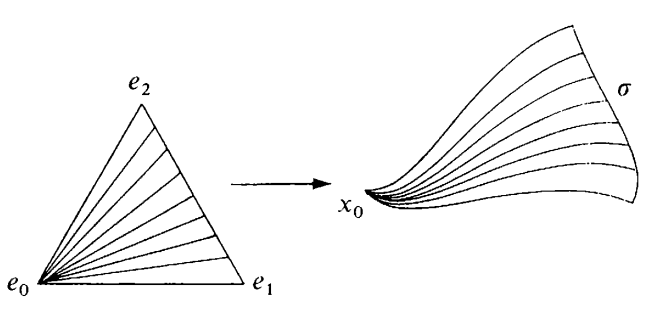
\includegraphics[width=0.8\textwidth]{Figures/cone-construction.png}
        \caption{The Cone Construction}
        \label{fig:Figures-cone-construction-png}
    \end{figure}

    This $D$ now extends to a homomorphism
    $D \colon \Delta_{n-1}(X) \to \Delta_n(X)$.\\
    \linebreak
    To compute the $i$ th face of the singular simplex
    $D \sigma$ for $i>0$, we put $\lambda_i = 0$ in
    \eqref{eq:B}, and we get
    $(D \sigma)^{(i)} = D \left( \sigma^{(i-1)} \right) $, and
    also
    $(D\sigma)^{(0)} = \sigma$.

    But now we find that when $n>1$,
    \[
    \partial \left( D \sigma \right) =
    \left( D \sigma \right)^{(0)}-
    \sum_{i=1}^{n} (-1)^{i-1} (D\sigma)^{(i)}
    = (D \sigma)^{(0)} - 
    \sum_{j=0}^{n-1} (-1)^{j} D (\sigma^{(j)}) = 
    \sigma - D\left( \partial \sigma \right) .
    \] 
    For $n=1$ (so when $\sigma$ is a $0$-simplex), we have
    \[
    \partial \left( D \sigma \right) =
    \sigma - \sigma_0, \quad \text{where } \sigma_0
    \colon \Delta_0 \to \left\{ x_0 \right\} .
    \] 
    and $D (\partial \sigma) = 0$ by definition.

    Thus $\partial D + D \partial = \id - \varepsilon$, where
    $ \varepsilon  \colon \Delta_i (X) \to 
    \Delta_i (X)$ is given by
    $ \varepsilon = 0$ for
    $i \neq 0$ and
    $\varepsilon \left( \sum n_{\sigma} \sigma \right) =
    (\left( \sum n_{\sigma} \right) \sigma_0$ for
    $i = 0$ and where
    $\sigma_0$ is the $0$-simplex at $x_0$.
    Thus, in homology,
    $\id = \id_* = \varepsilon_*$ which is
    $0$ in nonzero dimensions.
\end{proof}

\subsection{Cross Product}

We want to define a cross product
\[
\times  \colon \Delta_p (X) \times \Delta_q (Y)
\to \Delta_{p+q} (X \times Y).
\] 
If $x \in X$, we denote also by $x$ the singular
$0$-simplex sending $e_0$ to $x$.

Now for $\sigma \colon \Delta_q \to Y$, we let
$x \times \sigma$ be the singular $q$-simplex of
$X \times Y$ taking $w \mapsto (x, \sigma(w))$, and
similarly for $y \in Y$.
This defines $\times $ on 
$\Delta_0 (X) \times \Delta_q(Y)$ and
$\Delta_p(X) \times \Delta_0(Y)$.
We also define
$\times $ to be the zero map on elements
$(a,b)$ with either $a$ or $b$ being $0 \in 
\Delta_p(X) = \mathbb{Z}\Map (\Delta_p, X)$ or
$ 0 \in \Delta_q(Y) = \mathbb{Z}
\Map (\Delta_q, Y)$.

\begin{theorem}[]\label{Thm:LXOAUJC}
    There exist bilinear maps
    $\times  \colon \Delta_p(X) \times \Delta_q (Y)
    \to \Delta_{p+q}(X \times Y)$ such that:
    \begin{enumerate}
        \item for $x \in X, y \in Y, \sigma \colon
            \Delta_q \to Y$ and
            $\tau \colon \Delta_p \to X$,
            $x \times \sigma$ and $\tau \times y$ are as
            described above;
        \item (naturality) if $f \colon X \to X'$ and
            $g \colon Y \to Y'$, and if
            $f \times g \colon X \times Y \to 
            X' \times Y'$ denotes the product map, then
            \[
                (f \times g)_{\Delta} (a \times b)
                = f_{\Delta} (a) \times g_{\Delta}(b); \quad
                \text{and}
            \] 
        \item (boundary formula) $\partial (a \times b) =
            \partial a \times b + (-1)^{\deg a} a \times \partial b$.
    \end{enumerate}
\end{theorem}

\begin{proof}
    Note that $(3)$ holds when
    $p$ or $q$ is $0$.\\
    \linebreak
    
    The method of proof here goes by
    the name of "acyclic models". It can be made general, but
    we will just carry it out in the specific situation
    of our theorem.\\
    \linebreak
    Let $\id_p \colon \Delta_p \to \Delta_p$ be the
    identity map, thought of as a singular
    $p$-simplex of the space  $\Delta_p$.\\
    
    Let $p>0$ and $q>0$, and assume $\times $ has been
    defined for smaller $p+q$ satisfying the conditions above.\\
    The idea is to first define
    $\id_p \times \id_q$ on the "models".
    To do this, we first use (3) to compute that
    $\partial \left( \id_p \times \id_q \right) = 0$.
    Since $\Delta_p \times \Delta_q$ is contractible, we saw
    that $H_* \left( \Delta_p \times \Delta_q \right) = 0$, so
    $\partial \left( \id_p \times \id_q \right) $ is a 
    boundary of something. We let
    $\id_p \times \id_q$ denote this element. So
    $\partial \left( \id_p \times \id_q \right) =
    \partial \id_p \times \id_q +
    (-1)^{p} \id_p \times \partial \id_q$. Afterwards,
    we define $\sigma \times \tau$ in general by applying
    naturality (2) to maps
    $\sigma \colon \Delta_p \to X$ and
    $\tau \colon \Delta_q \to Y$.\\
    \linebreak
    To carry this out, we have
    \[
    \partial \left( \id_p \times \id_q \right) 
    = \partial \id_p \times \id_q + 
    (-1)^{p} \id_p \times \partial \id_q
    \in \Delta_{p+q-1}\left( \Delta_p \times \Delta_q \right) .
    \] 
    Now
    \[
    \partial (rhs) = 
    \partial \partial \id_p \times \id_q 
    +(-1)^{p-1} \partial \id_p \times \partial \id_q
    + (-1)^{p} \partial \id_p \times \partial \id_q
    +  \id_p \times \partial \partial \id_q = 0.
    \] 
    Hence the rhs is a $(p+q-1)$-cycle, so by the above,
    we can choose $\partial \left( \id_p \times \id_q \right) 
    = \partial \id_p \times \id_q + (-1)^{p} \id_p \times 
    \partial \id_q$.

    Now if $\sigma \colon \Delta_p \to X$ and
    $\tau \colon \Delta_q \to Y$ are arbitrary singular
    simplices, then
    regarding them also as maps which then
    induce homomorphisms of chain groups, we have
    $\sigma = \sigma_{\Delta}(\id_p)$ and
    $\tau = \tau_{\Delta}(\id_p)$.

    By (2), we must define
    $\sigma \times \tau = \sigma_{\Delta}(\id_p) \times 
    \tau_{\Delta}(\id_q) = 
    \left( \sigma \times \tau \right)_{\Delta}
    \left( \id_p \times \id_q \right) $.
    For $f \colon X \to X'$ and $g \colon Y \to Y'$, we 
    then have
    \begin{align*}
        (f \times g)_{\Delta}
        \left( \sigma \times \tau \right) 
        &= \left( f \times g \right)_{\Delta}
        \left( \sigma \times \tau \right)_{\Delta}
        \left( \id_p \times \id_q \right) 
        \\
        &= \left( f \circ \sigma \times g \circ \tau \right)_{\Delta}
        (\id_p \times \id_q)\\
        &= \left( f \circ \sigma \right)_{\Delta}(\id_p)
        \times \left( g \circ \tau \right)_{\Delta}
        (\id_q)\\
        &= f_{\Delta} (\sigma) \times 
        g_{\Delta}(\tau).
    \end{align*}
    Hence naturality (2) holds in general in these
    dimensions.

    For $(3)$, we have
    \begin{align*}
        \partial (\sigma \times \tau)
        &= \partial \left( \left( \sigma \times \tau \right)_{\Delta}
        \left( \id_p \times \id_q \right) \right) \\
        &= \left( \sigma \times \tau \right)_{\Delta}
        \left( \partial \left( \id_p \times \id_q \right)  \right) 
        \tag{Ch map commutes w $\partial$}\\
        &= \left( \sigma \times \tau \right)_{\Delta}
        \left( \partial \id_p \times \id_q +
        (-1)^{p} \id_p \times \partial \id_q \right) \\
        &= \partial \sigma_{\Delta}(\partial \id_p) \times 
        \tau_{\Delta}(\id_q) + (-1)^{p}
        \sigma_{\Delta}(\id_p) \times 
        \tau_{\Delta}\left( \partial \id_q \right) \\
        &= \partial \sigma \times \tau +
        (-1)^{p} \sigma \times \partial \tau,
    \end{align*}
    which extends to all chains by bilinearity.
\end{proof}

\begin{definition}[]
    If $(X,A)$ and $(Y,B)$ are pairs of spaces, then
    $(X ,A) \times (Y,B)$ denotes the pair
    $\left( X \times Y, 
    X \times B \cup  A \times Y\right) $.
\end{definition}

\begin{proposition}[]
    The cross product 
    $\Delta_p(X) \times \Delta_q (Y) \to 
    \Delta_{p+q}(X \times Y)$ induces a bilinear
    map $\times  \colon H_p (X,A) \times 
    H_q (Y,B) \to H_{p+q} \left( (X ,A) \times (Y,B) \right) $ 
    defined by $\left[ a \right] \times 
    \left[ b \right] = \left[ a \times b \right] $.
\end{proposition}

\begin{proof}
    If $a \in \Delta_p (X)$ with
    $\partial a \in \Delta_{p-1}(A)$ (i.e., represents
     a cycle of $(X,A)$) and
     $b \in \Delta_q(Y)$ with $\partial b \in \Delta_{q-1}(B)$, then
     \[
     \partial \left( a\times b \right) 
     = \partial a \times b + (-1)^{p} a \times \partial b
     \in \Delta_{p+q-1}\left( (A \times Y) \cup 
     (X \times B) \right) 
     \] 
     so
     $a \times b$ is a cycle in
     $\Delta_{p+q} \left( (X,A) \times (Y,B) \right) $.

     To show that it does not depend on the
     choices of representatives of relative homology classes,
     we note that if we add chains in $A$ or $B$, then
     these clearly vanish under $\partial$. Also,
     \begin{align*}
         (a+ \partial a') \times 
         (b + \partial b')
         &= a \times b + a \times \partial b' +
         \partial a' \times b + \partial a' \times \partial b'\\
         &= a \times b \pm \partial (a \times b')
         + \partial (a' \times b) +
         \partial (a' \times \partial b')
         + \left( \text{ch in } A \times Y \cup 
         X \times B\right)
     \end{align*}
     when $a$ and $b$ are relative cycles.
\end{proof}

\subsubsection{Proving that the Homotopy Axiom holds
for Singular Homology}

Let $X = I = \left[ 0,1 \right] $ and regard
also $I$ as the affine simplex
$\left[ \left\{ 0 \right\} ,\left\{ 1 \right\}  \right] 
\colon \Delta_1 \to I$ and let
$\varepsilon_0, \varepsilon_1$ be the $0$-similices
$\varepsilon_0 (e_0) = \left\{ 0 \right\} $ and
$\varepsilon_1 (e_0) = \left\{ 1 \right\} $ of $I$.
Then $\partial I = \varepsilon_1 - \varepsilon_0$.\\
\linebreak
Next, given a chain
$c \in \Delta_q (X)$, we have
$I \times c \in \Delta_{q+1}(I \times X)$, and
\[
\partial \left( I \times c \right) =
\partial I \times c - I \times \partial c
= \varepsilon_1 \times c - \varepsilon_0 \times c
- I \times \partial c.
\] 

Define $D \colon 
\Delta_q (X) \to \Delta_{p+1}(I \times X)$ by
$D(c) = I \times c$. Then
\[
    \left( \partial D + D \partial \right) (c)
    = \partial \left( D (c) \right) +
    D\left( \partial c \right) = 
    \varepsilon_1 \times c- \varepsilon_0 \times c.
\] 
Let $\eta_0$ and $\eta_1$ be the maps
$X \to I \times X$ given by
$\eta_0 (x) = (0,x)$ and $\eta_1 (x) = (1,x)$.
Then $\eta_{i \Delta}(c) = \varepsilon_i \times c$.
Thus
\[
\partial D + D \partial = 
\eta_{1 \Delta} - \eta_{0 \Delta}
\] 


\begin{theorem}[]
    If $f_0 \simeq f_1 \colon (X,A) \to (Y,B)$, then
    $f_{0 \Delta} \simeq f_{1 \Delta} \colon
    \Delta_* (X,A) \to \Delta_* (Y,B)$, and therefore
    $f_{0*} = f_{1*} \colon
    H_*(X,A) \to H_*(Y,B)$.
\end{theorem}

\begin{proof}
    Let $F \colon I \times (X,A) \to (Y,B)$ be a homotopy
    between $f_0$ and $f_1$, so $F \circ \eta_0 = f_0$ and
    $F \circ \eta_1 = f_1$, then 
    it induces
    $F_{\Delta} \colon \Delta_* \left( I \times X,
    I \times A\right) \to \Delta_*(Y,B)$. If we compose
    this with $\partial D + D \partial = 
    \eta_{1 \Delta} - \eta_{0 \Delta}$, we obtain
    \[
    \partial \left( F_{\Delta}\circ D \right) +
    \left( F_{\Delta}\circ D \right) \partial =
    F_{\Delta} \circ \left( \partial D + D \partial \right) 
    = F_{\Delta} \circ \eta_{1 \Delta} - 
    F_{\Delta} \eta_{0 \Delta}=
    f_{1 \Delta} - f_{0 \Delta},
    \] 
    showing that
    $F_{\Delta}\circ D$ is the desired chain homotopy.
    From this the second statement follows immediately.
\end{proof}

\begin{corollary}
    Singular homology satisfies the Homotopy Axiom.
\end{corollary}
















\begin{definition}[Graded group]
    A graded group is a collection of abelian groups
    $C_i$ indexed by the integers.
\end{definition}


\begin{definition}[Degree of map of graded groups]
Suppose $A_*, B_*, C_*$ and $D_*$ are graded groups.

A map $f \colon A_* \to B_*$ is said to be of degree
$d$ if it takes $A_i$ to $B_{i+d}$ for all $i$.
\end{definition}

We define
\[
    (A_* \otimes B_*)_n :=
    \bigoplus_{i+j=n} A_i \otimes B_j.
\] 

If $f \colon A_* \to C_*$ and $g \colon B_* \to D_*$, we
define
$f \otimes g \colon A_* \otimes B_* \to 
C_* \otimes D_*$ by
\[
    \left( f \otimes g \right) \left( a \otimes
    b\right) = (-1)^{\deg (a) \deg (g)} 
    f(a) \otimes g(b).
\] 

Then we obtain that
\begin{align*}
    \left( f \otimes g \right) \circ
    (h \otimes k) (a \otimes b) 
    &= (-1)^{\deg k \deg a} (f \otimes g) (h(a) \otimes k(b))\\
    &= (-1)^{\deg k \deg a + \deg g (\deg h + \deg a)}
    (f \circ h)(a) \otimes (g \circ k)(b)\\
    &= (-1)^{\deg k \deg a + \deg g(\deg h + \deg a) +
    (\deg g + \deg k) \deg a}
    (f \circ h) \otimes (g \circ k) (a \otimes b)\\
    &=  (-1)^{\deg g \deg h} (f \circ h ) \otimes 
    (g \circ k) (a \otimes b).
\end{align*}


In particular, for the chain complexes
$\Delta_*(X)$ and $\Delta_*(Y)$, we have the chain complex
\[
    \left( \Delta_*(X) \otimes \Delta_*(Y) \right)_n
    = \bigoplus_{i+j=n} \Delta_i (X) \otimes \Delta_j(Y),
\] 
with boundary operator $\partial_{\otimes} = 
\partial \otimes \id + \id \otimes \partial$, meaning
\[
\partial_{\otimes}\left( a_p \otimes b_q \right) 
= \partial a \otimes b + (-1)^{p} a \otimes \partial b
\] 
since $\id$ has degree $0$.
The subscript on $\partial_{\otimes}$ will often be dropped.

So now we have a chain complex
$\left( \Delta_*(X) \otimes \Delta_*(Y) ,
\partial_{\otimes } \right) $.

\begin{note}
    Note that
    if $x$ and $y$ are points, then
     $\left( \Delta_* (\left\{ x \right\} ) 
     \otimes \Delta_*\left( \left\{ y \right\}  \right) \right)_0
     = \Delta_0 \left( \left\{ x \right\}  \right) 
     \otimes \Delta_0 \left( \left\{ y \right\}  \right) 
     \cong \mathbb{Z}$ generated by
     $x \otimes y$ and
     $\Delta_0 \left( \left\{ x \right\} \times 
     \left\{ y \right\} \right) \cong \mathbb{Z}$ generated
     by $(x,y)$.
\end{note}

We ask whether this always works.

Recall the cross product defined on
chain complexes:
\[
\times \colon \Delta_*(X) \times \Delta_*(Y) \to 
\Delta_*(X \times Y).
\] 
Since it was bilinear, it induces a homomorphism
\[
\times \colon \Delta_*(X) \otimes \Delta_*(Y) \to 
\Delta_*(X \times Y)
\] 
which, by definition, takes
$a \otimes b$ to $a \times b$.

By Theorem \ref{Thm:LXOAUJC}, the
product is natural in $X$ and $Y$, and when
$X$ and $Y$ are points, it is the canonical map
$x \times y = (x,y)$, and also the boundary formula
$\partial \left( a \times b \right) =
\partial a \times b + (-1)^{\deg a} a \times \partial b$ holds.

Thus
\begin{align*}
    \partial \left( \times (a \otimes b) \right) 
    &= \partial (a \times b) = 
    \partial a \times b + (-1)^{\deg a} a \times \partial b\\
    &= \times  \left( \partial a \otimes b+
    (-1)^{\deg a} a \otimes \partial b\right) \\
    &= \times \left( \partial_{\otimes} 
    (a \otimes b)\right) .
\end{align*}
So $\times $ is a chain map 
$\left( \Delta_{*}(X) \otimes \Delta_*(Y), \partial_{\otimes}
\right) \to 
\left( \Delta_*(X \times  Y), \partial \right) $.

\begin{lemma}[]
    If $X$ and $Y$ are contractible, then there is a chain
    contraction of
    $\Delta_*(X) \otimes \Delta_*(Y)$. Consequently,
    $H_n\left( \Delta_*(X) \otimes \Delta_*(Y) \right) = 0$ for
    $n>0$ and is $\mathbb{Z}$, generated by
    $\left[ x_0 \otimes y_0 \right] $, for $n=0$.
\end{lemma}

\begin{proof}
    In Theorem \ref{Thm:OOCPPX}, we constructed a
    chain contraction for $X$. I.e., we
    constructed a map $D \colon \Delta_p(X) \to 
    \Delta_{p+1}(X)$ such that
    $\partial D + D \partial = \id - \varepsilon$ - where
    $\varepsilon$ is the augmentation map.

    Let $E = 
    D \otimes \id + \varepsilon \otimes D$ on
    $\Delta_*(X) \otimes \Delta_*(Y)$. Then

    \begin{align*}
        E \partial_{\otimes} + 
        \partial_{\otimes} E 
        &= (D \otimes \id + \varepsilon \otimes D)
        \left( \partial \otimes \id + \id \otimes \partial \right) 
        + \left( \partial \otimes \id + \id \otimes
        \partial \right) \left( D \otimes \id + \varepsilon
        \otimes D\right) \\
        &= (-1)^{\deg \id \deg \partial }
        D \partial \otimes \id
        + (-1)^{\deg id \deg id}D \otimes \partial 
        + (-1)^{\deg D \deg \partial} \varepsilon \partial
        \otimes D\\ 
        &+ (-1)^{\deg D \deg \id}
        \varepsilon \otimes D \partial 
        + (-1)^{\deg id \deg D} \partial D \otimes \id
        + (-1)^{\deg \id \deg \varepsilon}
        \partial \varepsilon \otimes D \\
        &+ (-1)^{\deg \partial \deg D}
        D \otimes \partial
        +
        (-1)^{\deg \partial \deg \varepsilon}
        \varepsilon \otimes \partial D \\
        &= D \partial \otimes \id
        + \varepsilon \otimes D \partial
        + \partial D \otimes \id
        + \varepsilon \otimes \partial D
    \end{align*}
    Note that we here have used that $\varepsilon$ is a chain
    map, but $D$ might not be which is why the
    terms above survive.
    Now
    \begin{align*}
        D \partial \otimes \id + \varepsilon \otimes D \partial
        + \partial D \otimes \id + \varepsilon \otimes \partial D
        &= (\id - \varepsilon - \partial D)
        \otimes \id + \varepsilon \otimes
        (\id - \varepsilon - \partial D)
        + \partial D \otimes \id + \varepsilon \otimes
        \partial D\\
        &= \id \otimes \id 
        - \varepsilon \otimes \varepsilon \\
    \end{align*}
\end{proof}

\begin{theorem}[]
    There exists a natural (in $X$ and $Y$ ) chain
    map
    \[
    \theta \colon \Delta_* (X \times Y) \to 
    \Delta_* (X) \otimes \Delta_*(Y)
    \] 
    which is the canonical map $(x,y) \mapsto x \otimes y$ in
    degree $0$.
\end{theorem}

\begin{proof}
    The proof is simple and by acyclic models. See
    Bredon's book.
\end{proof}

\begin{theorem}[]
    Any two natural chain maps on
    $\Delta_*(X \times Y)$ to itself or on
    $\Delta_* (X) \otimes \Delta_*(Y)$ to itself or
    on one of these to the other which are the
    canonical isomorphisms in degree zero, with $X$ and
    $Y$ points, are naturally chain homotopic.
\end{theorem}

\begin{corollary}[The Eilenberg-Zilber Theorem]
    The chain maps
    \[
    \theta \colon \Delta_* (X \times Y) \to 
    \Delta_*(X) \otimes \Delta_*(Y)
    \] 
    and
    \[
    \times \colon \Delta_*(X) \otimes \Delta_*(Y)
    \to \Delta_*(X \times Y)
    \] 
    are natural homotopy equivalences which are naturally
    homotopy inverses of one another.
\end{corollary}

\begin{corollary}
    \[
    H_p(X \times Y; G) \cong
    H_P\left( \Delta_*(X) \otimes
    \Delta_*(Y) \otimes G\right) ,
    \] 
    and
    \[
    H^{p}\left( X \times Y;G \right) 
    \cong H^{p}\left( \Hom \left( 
    \Delta_*(X) \otimes \Delta_*(Y) \right) ,G \right) 
    \] 
\end{corollary}

\begin{theorem}[Algebraic Künneth Theorem]
    Let $K_*$ and $L_*$ be free chain complexes.
    Then there is a natural exact sequence
    \[
    0 \to 
    \left( H_* (K_*) \otimes H_*(L_*) \right)_n 
    \stackrel{\times }{\to} H_n(K_* \otimes L_*)
    \to \left(\Tor
    \left( H_*(K_*), H_*(L_*) \right) \right)_{n-1} \to 0
    \] 
    which splits non-naturally.
\end{theorem}

\begin{note}
    Here
    \[
        \left( \Tor(A_*,B_*) \right)_{n}
        = 
        \bigoplus_{i+j=n}
        \Tor(A_i,B_j)
    \] 
\end{note}

\begin{theorem}[Geometric Künneth Theorem]
    There is a natural exact sequence
    \[
    0 \to \left( H_*(X) \otimes
    H_n(Y) \right)_n \stackrel{\times }{\to} 
    H_n(X \times Y) \to 
    \left( \Tor\left( H_*(X), H_*(Y) \right) \right)_{n-1}
    \] 
    which splits non-naturally.
\end{theorem}






    %\printbibliography
\end{document}
